\documentclass[12pt]{article}
\usepackage[top=0.9in, bottom=0.9in, left=0.9in, right=1.1in]{geometry}

\usepackage{graphicx,color,enumitem}
\usepackage{amsmath,amsthm,amsbsy}
\usepackage{palatino}
\usepackage{mdframed}

\usepackage{tikz}
\usepackage[colorlinks=true]{hyperref}

%% Setup aproblem environment, 
%% aproblem items
%% subproblems environment
%% subproblem items
\makeatletter
\newcounter{probcount}
\newcounter{subprobcount}
\newlength\probsep
\newlength\pshrinking
\newif\iffirstprob

\newenvironment{aproblems}%
  {\ifhmode\unskip\par\fi\setcounter{probcount}{0}\probsep\parskip
  \sbox\@tempboxa{\textbf{9.}}\pshrinking\wd\@tempboxa\advance\pshrinking\labelsep
  \let\hproblem\aproblem
  \advance\linewidth -\pshrinking
  \advance\@totalleftmargin\pshrinking
  \advance\leftskip\pshrinking}%
  {\ifhmode\unskip \par\fi\advance\leftskip-\pshrinking}%

\newcommand{\aproblem}{%
  \setcounter{subprobcount}{0}%
  \stepcounter{probcount}%
  \def\@currentlabel{\arabic{probcount}}%
  \ifhmode
    \unskip \par
  \fi
%  \addpenalty{-4000}%
  \iffirstprob\else\addvspace\probsep\fi
  \firstprobfalse
  \hskip -\labelwidth\hskip -\labelsep 
  \hbox to\labelwidth{\hss\textbf{E\arabic{probcount}.}}\hskip\labelsep
}%

\newcommand{\subprob}{\item\def\@currentlabel{\arabic{probcount}\alph{\thelistlabel}}}
\newcommand{\skipproblem}{\stepcounter{probcount}}


%% The following commands put defined left and right headers on the top, and a page number
%% on the bottom of all pages beyond page 1
\usepackage{fancyhdr}
\pagestyle{fancy}
\fancyfoot[C]{\ifnum \value{page} > 1\relax\thepage\fi}
\fancyhead[L]{\ifx\@doclabel\@empty\else\@doclabel\fi}
\fancyhead[R]{\ifx\@docdate\@empty\else\@docdate\fi}
\headheight 15pt
\def\doclabel#1{\gdef\@doclabel{#1}}
\def\docdate#1{\gdef\@docdate{#1}}
\makeatother

\mdfdefinestyle{probSty}{}
\theoremstyle{definition}
\newmdtheoremenv[style=probSty, linewidth=0.5pt, topline=false, bottomline=false, %
rightline=false, leftmargin=0pt, innerleftmargin=0.4em, rightmargin=0pt, %
innerrightmargin=0pt, innertopmargin=-5pt, innerbottommargin=3pt, %
splittopskip=\topskip, splitbottomskip=0.3\topskip, %
skipabove=1.3\topsep]{prob}{Problem}

\renewcommand*{\theprob}{\arabic{prob}}

%% General formatting parameters
\parindent 0pt
\parskip 6pt plus 1pt

%\newcommand{\prob}[1]{\noindent \textbf{Problem #1.} \,}
%\newcommand{\epart}[1]{\noindent \textbf{(#1)} \,}
\newcommand{\eps}{\epsilon}

\doclabel{Math F302 Homework 5.3}
\docdate{revised version; 4 November 2023}

\begin{document}
\renewcommand{\d}{\displaystyle}

\strut
\centerline{{\Large \textbf{Homework 5.3}}}

\bigskip
\centerline{{\large due 11:59pm Monday 6 November (\emph{revised}), by Gradescope as usual}}

\bigskip
\centerline{{\large \underline{all} of these exercises will be graded for correctness}}

\begin{quote}
\emph{This is a coherent story, with mixed-in problems that you should solve, that replaces the book's exercises for Section 5.3.  Please write your answers on a separate sheet, and clearly label you answers with ``Problem 1'' though ``Problem 9''.  Scan and turn in via gradescope as usual.}
\end{quote}

\noindent
\subsection*{Energy is just a technique for solving differential equations}

It is common to talk about natural gas or oil as ``energy.''   We say batteries use chemicals to store ``energy'' which they then deliver as electrical ``energy.''  People who know no physics or math happily discuss the ``energy industry'' and the ``politics of renewable energy''.

But this use of the word ``energy'' is new, younger than the United States of America.  It arose in physics before entering everyday language:

\small

\begin{quotation}
\noindent \emph{In 1807, Thomas Young was possibly the first to use the term ``energy'' \dots in its modern sense.  \dots  The law of conservation of energy was also first postulated in the early 19th century \dots}

\hfill \url{https://en.wikipedia.org/wiki/Energy}
\end{quotation}

\normalsize
Energy is an incomplete solution of a differential equation (DE) which describes some motion.  Its physical interpretation is as a conserved quantity that cannot be created or destroyed but only transformed.

From the point of view of Newtonian and classical mechanics, energy is a \emph{first integral} of the standard second-order DE for acceleration:
\begin{equation}
    mx''=F(x)  \label{Newton2nd}
\end{equation}
Here $x(t)$ is the position (trajectory) of a particle.  As shown below, the energy appears when you use a kind of integrating-factor technique for \eqref{Newton2nd}.  Notice that the force $F$ here depends only on the position $x$ and not on the velocity $x'$.

Finding the energy does not fully solve the DE.  However, it identifies a \emph{conserved quantity} for solutions, increasing understanding of the DE.  Though most DE textbooks discuss energy, ours does not.  This Homework introduces energy, and fixes the book's omission.

\medskip
\textbf{The energy and the first integral.}  To make the appearance even simpler, consider a second-order and possibly nonlinear DE of the form
\begin{equation}
y'' = f(y). \label{basicform}
\end{equation}
Equation \eqref{basicform} is basically the same as \eqref{Newton2nd}, but written to de-emphasize the connection with physics.

The solution of \eqref{basicform} is an unknown function $y(t)$.    Note that $y'$ does not appear in \eqref{basicform}.  The function $f(y)$ may be linear or nonlinear.

\begin{prob}
Find the general solution of \eqref{basicform} if $f(y)$ is the linear function
    $$f(y) = -ky - g$$
where $k$ and $g$ are positive real constants.  (\emph{Hint.}  An easy \S 4.3 and 4.4 problem.)
\end{prob}

We want to make progress solving DE \eqref{basicform}, that is, we want to \emph{integrate}.  But the right side of \eqref{basicform} is not a derivative of anything.  However, if we multiply both sides by $y'$ then both sides are derivatives:
\begin{align}
y' y'' &= y' f(y) \label{stepone} \\
\left(\frac{1}{2} (y')^2\right)' &= - \left(P(y)\right)'  \label{steptwo}
\end{align}
Here $P(z)$ is a function whose derivative is $-f(z)$:
    $$P'(z)=-f(z) \quad \text{ or } \quad P(z) = -\int f(z)\,dz.$$
The extra minus sign is merely traditional.  Notice that going from \eqref{steptwo} back to \eqref{stepone} requires the chain rule because $y=y(t)$.

\begin{prob}
To show that you understand the chain rule and antiderivative, as they relate to equations \eqref{stepone} and \eqref{steptwo}, do these basically meaningless calculations:
\renewcommand{\labelenumi}{\roman{enumi})}
\begin{enumerate}
\item simplify $\left(\frac{1}{7} (y')^7\right)'$ assuming $y(t)$ is some function.
\item find $P(z)$ if $f(z)=z-e^{-3 z}$.
\end{enumerate}
\end{prob}

Now that both sides of \eqref{steptwo} are derivatives, we can integrate both sides.  With slight re-arrangement we get
\begin{equation}
  \frac{1}{2} (y')^2 + P(y) = C  \label{basicfirstint}
\end{equation}
where $C$ is a constant of integration.  Equation \eqref{basicfirstint} is called the \emph{first integral} of DE \eqref{basicform}.  Note that it is a first-order nonlinear ODE which is a partial solution of \eqref{basicform}.  The left side of \eqref{basicfirstint} is called the \emph{energy} of DE \eqref{basicform}, a function of $y'$ and $y$:
\begin{equation}
  E(y,y') = \frac{1}{2} (y')^2 + P(y).  \label{basicenergydefn}
\end{equation}

\begin{prob}
Compute the energy and first integral if $f(y)=-ky-g$ as in Problem 1.
\end{prob}

The constant $C$ in equation \eqref{basicfirstint} can be evaluated from an initial condition.  For instance, for the initial value problem
    $$y''=f(y), \qquad y(0)=y_0, \quad y'(0)=v_0$$
we can use \eqref{basicfirstint} to find
    $$C = \frac{1}{2} (v_0)^2 + P(y_0).$$
Thus $C$ is the value of the energy at any time,
    $$E(y(t),y'(t)) = C.$$
The energy is a constant independent of $t$, unchanged from its initial value, if $y(t)$ is a solution of \eqref{basicform}.  This is what it means to say that \emph{energy is conserved}.

\medskip
\textbf{Energy in physics, and conservative forces.}  Now we return to the Newtonian equation \eqref{Newton2nd}, namely $m x'' = F(x)$.  Here the unknown solution is the position function $x(t)$.  As usual, $m$ is the (constant) \emph{mass} and the function $F$ is the \emph{force}.

The \emph{(total) energy} for equation \eqref{Newton2nd} is
\begin{equation}
  E(x,x') = \frac{1}{2} m (x')^2 + P(x)  \label{energydefn}
\end{equation}
where $P(x)$ is some antiderivative of $-F$:
\begin{equation}
P'(x)=-F(x).  \label{potentialfunction}
\end{equation}
Showing that \eqref{energydefn} follows from \eqref{Newton2nd} is the same calculation as showing how \eqref{basicenergydefn} is derived from \eqref{basicform}.

The energy is the sum of two parts, the \emph{kinetic energy} $\frac{1}{2} m (x')^2$ and the \emph{potential energy} $P(x)$.  The potential energy function $P(x)$ depends on position only and not velocity $x'$.  Regarding the sign choice in \eqref{potentialfunction}, this is simply a physics convention that the force is chosen to point down-slope (not up-slope) on the potential: $F(x)=-P'(x)$.  Such a force, which is the (negative) derivative of some potential energy, is called a \emph{conservative} force.  The forces of gravity and springs are conservative forces.

Drag forces from air resistance, or fluid damping forces, as appeared in some problems in sections 1.3, 3.1, 3.2, and 5.1, are \emph{not} conservative forces.  They are proportional to the velocity $x'$ or a power thereof, and they \emph{dissipate} energy as heat.  That is, when there is drag or damping then the sum of kinetic plus potential energy for the moving particle is not conserved but rather decreases in time.\footnote{However, microscopically, the energy of the huge system consisting of all the moving particles in the air (or fluid) would be conserved if it were isolated.}

\medskip
\textbf{A nonlinear spring.}  A linear spring, as described in section 5.1, is modeled by Hooke's law.  It applies force $F(x)=-kx$ when $x$ is the displacement from the relaxed position $x=0$.  However, as discussed in section 5.3, one may model more realistic nonlinear spring behavior by adding a term proportional to $x^3$.  For example, the force might be $F(x)=-k(x + \eps x^3)$ so that the equation of motion for a mass $m$ attached to a nonlinear spring might would be
\begin{equation}
m x'' = - k (x + \eps x^3) \label{nlspring}
\end{equation}
where $k>0$ is constant.  We will assume that $\eps>0$.  (This ``hard'' spring strongly resists compression/expansion too far from the relaxed position.)

\begin{prob}
Compute the energy $E(x,x')$ for DE \eqref{nlspring}.
\end{prob}

One can show a contour plot of the energy.  The non-intersecting contours show the possible motions, and the energy is constant along each contour.  Figure 1 shows such a plot.

\begin{figure}[h]
\begin{center}
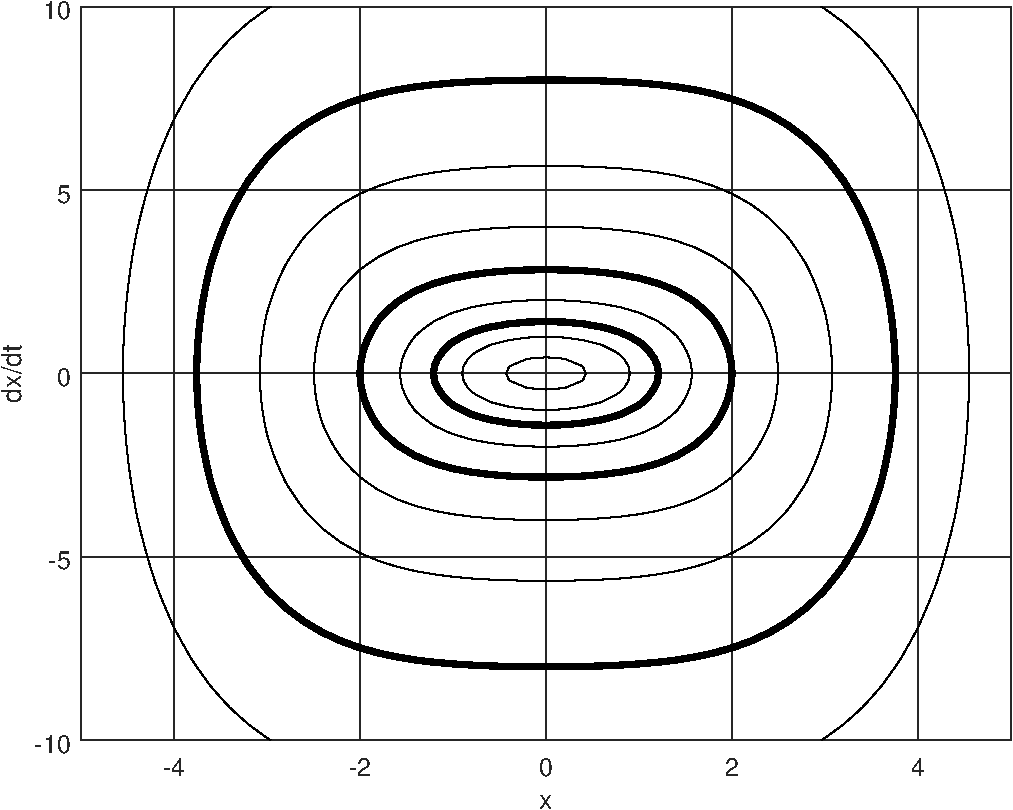
\includegraphics[width=0.75\textwidth]{figs/nlspringcurves.pdf}
\end{center}

\vspace{-5mm}
\caption{Contour plot of the energy $E(x,x')$ of a nonlinear spring.}
\end{figure}

\begin{prob}
I set $m=1$, $k=1$, and $\eps=\frac{1}{2}$ in equation \eqref{nlspring} when creating Figure 1.  Using your result from Problem 4 you have a particular energy function $E(x,x')$ of which Figure 1 is the contour plot.  Label the three bold contours in Figure 1 with the value of the energy.  Note these labels are \emph{specific numbers}, though some approximation is appropriate.
\end{prob}

\begin{prob}
Now assume the ODE is $y''=f(y)$, namely equation \eqref{basicform}, and that $f(y)=-ky-g$ as in Problems 1 and 3.  If $E(y,y')$ is the energy computed in Problem 3, what kinds of curves in the $y,y'$ plane are the equations $E(y,y')=C$?  Assuming $k=1$ and $g=10$, plot the (nonempty) curves in the $y,y'$ plane corresponding to three values of $C$ of your choice.  (\emph{You may use a computer to plot the curves, but it is not necessary.})  For what value of $C$ does the curve consist of a single point?  Interpret this single-point case.
\end{prob}

\medskip
\begin{minipage}[t]{0.65\textwidth}
\textbf{A pendulum.}  The figure at right shows a pendulum of mass $m$ attached to a rod of length $\ell$.  Gravity pulls straight down on the mass with force $-mg$ so that, as explained in section 5.3, the equation of motion is
\begin{equation}
m \ell \ddot{\theta} = -m g \sin\theta  \label{pendulum}
\end{equation}
Here we denote the time derivative with a dot.

\end{minipage}
\begin{minipage}[t]{0.35\textwidth}
\vspace{0pt}

\hfill 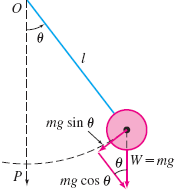
\includegraphics[width=0.8\textwidth]{figs/pendulum}
\end{minipage}

\begin{prob}
Compute the energy $E(\theta,\dot\theta)$ for DE \eqref{pendulum}.
\end{prob}

Figure 2 shows a contour plot of the energy $E(\theta,\dot\theta)$ for \eqref{pendulum} in the case where $m=1$ kg, $\ell=1$ m, and $g=10 \, \text{m}\,\text{s}^{-2}$. 

\begin{prob}
Label the bold contours in Figure 2 with the value of the energy; these labels are \emph{specific numbers} but some approximation is needed.  Interpret these bold contours and their energy values in terms of the behavior of the pendulum.  (\emph{Hint}:  There is no ceiling in the model.)  What is happening near the location $(\theta,\dot\theta)=(3.2,0)$?
\end{prob}

\begin{figure}[h]
\begin{center}
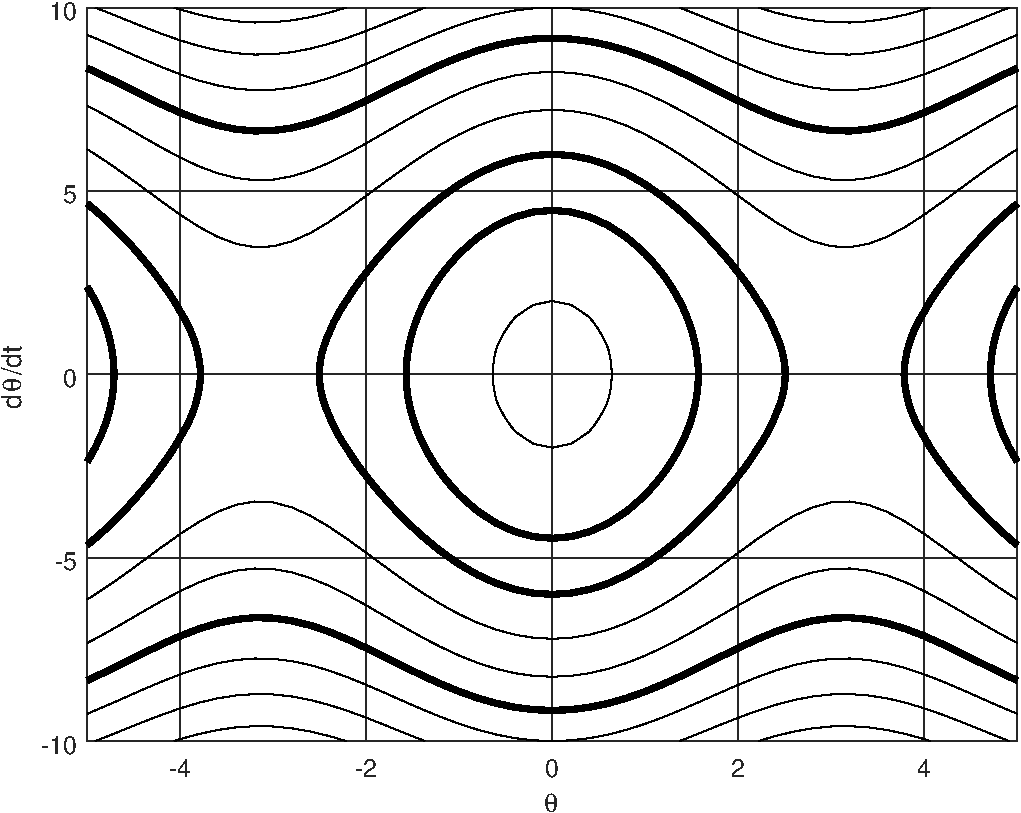
\includegraphics[width=0.75\textwidth]{figs/pendulumcurves}
\end{center}

\vspace{-5mm}
\caption{Contour plot of the energy $E(\theta,\dot\theta)$ of a pendulum.}
\end{figure}

\medskip
\textbf{Solving certain nonlinear 2nd-order ODEs.}  Recall that any 2nd-order ODE can be written in the \emph{normal form} mentioned in section 1.1,
    $$y'' = f(t,y,y').$$
Such a general ODE is often too difficult to solve.  However, if variables are \textbf{missing from the right side function $f$} then one can exploit that to solve the equation.  For example
    $$y'' = f(y')$$
can be solved, at least partially, by recognizing that it is first-order \emph{for the derivative} $y'$.  That is, one can substitute $u=y'$ and attempt to solve the first-order ODE $u'=f(u)$.  This equation is separable: \, $\frac{du}{dt} = f(u) \, \iff \, \int \frac{du}{f(u)} = \int dt = t + c$.

The table below lists some cases where one can make progress on nonlinear 2nd-order ODEs, supposing one can compute an integral.  Energy fits in this framework.

\medskip
\begin{tabular}{c|l|l}
DE & technique & first integral \\ \hline \hline
$y'' = f(t,y,y')$ & \emph{too general!} & \emph{generally no first integral} \\ \hline
$y'' = f(t)$ & just antidifferentiate & $y' = F(t)+c \large\strut$\, where $F(t) = \int f(t)\,dt$ \\ \hline
$y'' = f(y)$ & compute energy & $\frac{1}{2} (y')^2 + P(y) = c \large\strut$\, where $P(z) = -\int f(z)\,dz$ \\ \hline
$y'' = f(y')$ & substitute $u=y'$ & $Q(y') = t + c \large\strut$\, where $Q(u)=\int \frac{du}{f(u)}$
\end{tabular}

\medskip
\begin{prob}
Solve the initial value problem:
    $$y'' = - (y')^3, \qquad y(1)=5, \quad y'(1)=\frac{1}{2}$$
\end{prob}

\end{document}
